	In many machining cases, orthogonal cutting may be considered a good approximation to perform on the major cutting edge, that is why it has been extensively studied \cite{shaw2005metal}. For instance, planing and facing processes are some examples that orthogonal cutting conditions can be observed.

	Also, it is known that thermal behavior during the cutting process, as temperature fields and heat flows, has a important influence on tool life, surface finish and metallurgical structure of workpiece and machinability. Then, the study of thermal analysis on orthogonal cutting case shall be able to provide a better comprehension of many studies concerning thermal modeling of metal cutting processes \cite{komanduri2000thermal}, \cite{komanduri2001thermal}.
	
	\section{Principles of metal cutting}
	write

	\section{Mechanics of orthogonal cutting}

	In this paper it will be show numerous correlations among forces, stresses and dimensions for example. For this purpose it is important to discuss about geometrical correlations in the composite cutting force circle (figure \ref{fig:circlec}).

	\begin{figure}[h]
		\centering
		\captionsetup{justification=centering}
		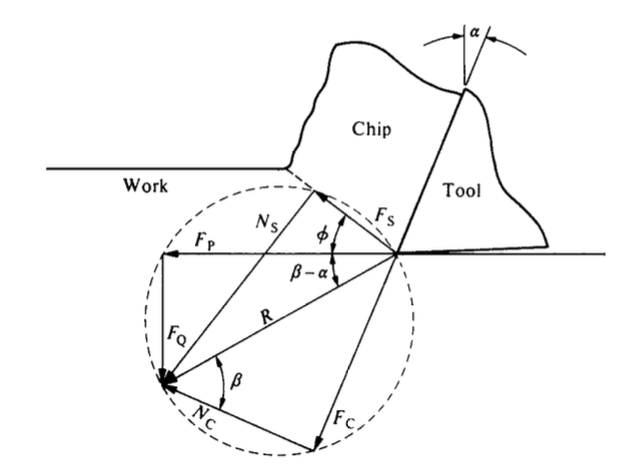
\includegraphics[scale=0.5]{Cap1/circlec.png}
		\caption{Cutting forces \cite{shaw2005metal}}
		\label{fig:circlec}
	\end{figure}

	From the figure \ref{fig:circlec} it can be stated about forces on the primary shear zone reference $F_{S}$ and $N_{S}$:

	\begin{equation} 
	\label{}
	F_{S} = F_{P}\cos\phi - F_{Q}\sin\phi
	\end{equation}
	\begin{equation} 
	\label{}
	N_{S} = F_{Q}\cos\phi + F_{P}\sin\phi
	\end{equation}

	Also for the forces on the chip flow reference:

	\begin{equation} 
	\label{}
	F_{C} = F_{P}\sin\alpha + F_{Q}\cos\alpha
	\end{equation}
	\begin{equation} 
	\label{}
	N_{C} = F_{P}\cos\alpha - F_{Q}\sin\alpha
	\end{equation}

	These equation provide all auxiliar forces related to the known passive force $F_{Q}$ and force on the cutting direction $F_{P}$. Now, the variables of interest can be easily calculated, as the friction coefficient:

	\begin{equation} 
	\label{eq_friction}
	\mu = \frac{F_{C}}{N_{C}} = \frac{F_{Q} + F_{P}\tan\alpha}{F_{P} - F_{Q}\tan\alpha}
	\end{equation}

	Now the equations concerning about stresses are:

	\begin{equation} 
	\label{}
	A_{S} = \frac{wa_{p}}{\sin\phi}
	\end{equation}

	\begin{equation} 
	\label{}
	\tau = \frac{F_{S}}{A_{S}} = \frac{(F_{P}\cos\phi - F_{Q}\sin\phi)\sin\phi}{wa_{p}}
	\end{equation}

	\begin{equation} 
	\label{}
	\sigma = \frac{N_{S}}{A_{S}} = \frac{(F_{P}\sin\phi + F_{Q}\cos\phi)\sin\phi}{wa_{p}}
	\end{equation}

	Where $A_{S}$ is the area of the shear plane, $\tau$ is the shear stress and $\sigma$ is the normal stress.

	Another important parameter is the cutting ratio $r$, which can provide an important relation between the main cutting velocity and the chip outlet velocity. It is found experimentally that there is no change in density of metal during the cutting process and also for $w/a_{p} \geq 5$ the width of the chip is the same of the workpiece. Then, the equations are:

	\begin{equation} 
	\label{}
	a_{p}wl = a_{pc}w_{c}l_{c}
	\end{equation}

	Where $a_{p}$, w and l are the depth of cut, width of cut and length of cut respectively. Then, the cutting ratio is defined by:

	\begin{equation} 
	\label{}
	r = \frac{a_{p}}{a_{pc}} = \frac{l_{c}}{l}
	\end{equation}

	Having the cutting ratio, it is now possible to correlate cutting velocity $v$ and chip outlet velocity $v_{c}$ by means of the following equation:

	\begin{equation} 
	\label{}
	v_{c} = rv
	\end{equation}
	
	\section{Objective}

	The aim of this paper is to develop a computational method to analyze thermal images generated during the orthogonal cutting of AISI 1045 metal, focusing on the transient state due to the short time of cutting. It will be analyzed temperature distribution along the cutting tool, heat flows through tool, chip and workpiece.

	\section{Structure}
	
	This work is divided into 6 Chapters, including this \textbf{\nameref{ch:intro}}, plus one Appendix.
	
	The second chapter, \textbf{\nameref{ch:state}}, describes the existing technology which is relevant for the scope of this paper and upon which the work was built.

	The third chapter, \textbf{\nameref{ch:setup}}, describes the methodology and materials that conducted the experiments.
	
	The fourth, \textbf{\nameref{ch:implementation}}, describes the logical implementation of the final analysis code.
	
	The fifth, \textbf{\nameref{ch:results}}, presents the results and discussions about the outputs of the final code.
	
	The sixth and final chapter, \textbf{\nameref{ch:conclusions}}, sums up what was accomplished in this work and suggests how it may be expanded for new processes.
	
	The Appendix~\textbf{\nameref{ch:code}} contains all the code written for the program.